\subsection{Entwurfsmuster}

\subsubsection{MatFlow}
MatFlow, wie schon im Kommunikationskapitel gesehen, ist eine Schichtenarchitektur, die über Fassaden miteinander verbunden ist
(\nameref{API} und Database package)

\subsubsection{\nameref{API}}
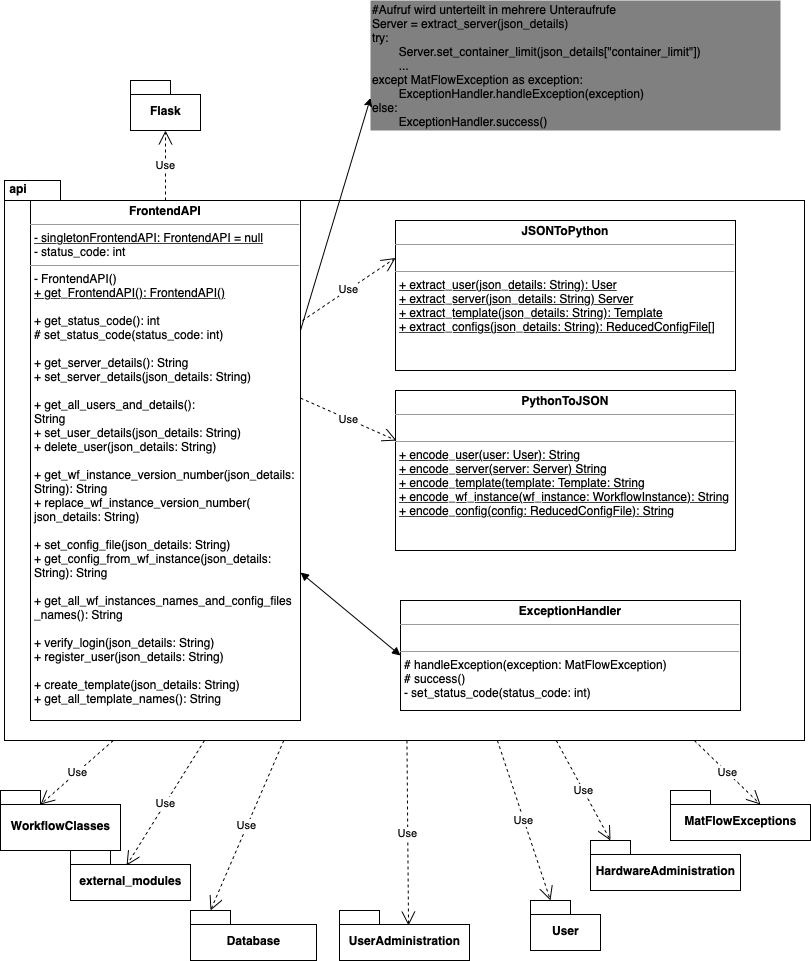
\includegraphics[width=1\textwidth]{res/api.drawio.png}
Hier ist die Klasse FrontendAPI die eigentliche Fassade. Der Grund dafür ist womögliche Abhängigkeiten zwischen
der Client Applikation und der Serverapplikation zu entkoppeln. Sie wurde als Singleton implementiert, da die API
nur auf einem Port auf dem Server laufen soll und global ansprechbar sein soll. Mehrere essentiell gleiche APIs auf
verschiedenen Ports wären uneindeutig.


\newpage